\textbf{- Reference:} 
\href{https://www.zama.ai/post/tfhe-deep-dive-part-2}{TFHE Deep Dive - Part II - Encodings and linear leveled operations}~\cite{tfhe-2}

$ $

Suppose we have a GLWE ciphertext $C$:

$C = \textsf{GLWE}_{S, \sigma}(M) = ( A_1, A_2, ... \text{ } A_{k-1}, B) \in \mathcal{R}_{\langle n,q \rangle}^{k + 1}$

$ $

\noindent and a new plaintext polynomial $\Lambda$ as follows: 

$\Lambda = \sum\limits_{i=0}^{n-1}(\Lambda_i \cdot X_i) \in \mathcal{R}_{\langle n, q \rangle}$

$ $

\noindent Let's define the following ciphertext-to-plaintext multiplication operation:

$\Lambda \cdot C = (\Lambda \cdot A_0, \Lambda \cdot A_1, ... \text{ } \Lambda \cdot A_{k-1}, \Lambda \cdot B)$

$ $

\noindent We assume that we always do polynomial-to-polynomial multiplications efficiently in $O(n \log n)$ by using the NTT technique (\autoref{sec:ntt}). Then, the following is true: 

\begin{tcolorbox}[title={\textbf{\tboxlabel{\ref*{sec:glwe-mult-plain}} GLWE Ciphertext-to-Plaintext Multiplication}}]
$\Lambda \cdot \textsf{GLWE}_{S, \sigma}(\Delta M)$

$= \Lambda \cdot (\{A_i^{\langle 1 \rangle}\}_{i=0}^{k-1}, \text{ } B^{\langle 1 \rangle})$

$= (\{\Lambda\cdot A_i^{\langle 1 \rangle}\}_{i=0}^{k-1}, \text{ } \Lambda \cdot B^{\langle 1 \rangle})$

$= \textsf{GLWE}_{S, \sigma}(\Delta (M \cdot \Lambda) )$
\end{tcolorbox}

This means that multiplying a plaintext (polynomial) by a ciphertext (polynomial) and decrypting it gives the same result as multiplying the two original plaintext polynomials.  

$ $

%\noindent \textbf{\underline{Proof}}
\begin{myproof}
\begin{enumerate}
\item Define the following notations: \\
$A_1' = \Lambda \cdot A_1$ \\
$A_2' = \Lambda \cdot A_2$ \\
$...$ \\
$A_{k-1}' = \Lambda \cdot A_{k-1}$ \\
$E' = \Lambda \cdot E$ \\
$B' = \Lambda \cdot B$ \\
\item Derive the following: \\
$B' = \Lambda \cdot B$ \\
$= \Lambda \cdot (\sum\limits_{i=0}^{k-1}{(A_i \cdot S_i)} + \Delta \cdot M + E)$ 
$= \sum\limits_{i=0}^{k-1}{(\Lambda \cdot A_i \cdot S_i)} + \Delta \cdot \Lambda \cdot M + \Lambda \cdot E$   \\ \textcolor{red}{ \# by the distributive property of a polynomial ring} \\
$= \sum\limits_{i=0}^{k-1}{((\Lambda \cdot A_i) \cdot S_i)} + \Delta \cdot (\Lambda \cdot M) + (\Lambda \cdot E)$  \\
$= \sum\limits_{i=0}^{k-1}{(A_i' \cdot S_i)} + \Delta \cdot (\Lambda \cdot M) + (E')$ \\
\item Since $B' = \sum\limits_{i=0}^{k-1}{(A_i' \cdot S_i)} + \Delta \cdot (\Lambda \cdot M) + (E')$, 

$(A_1', A_2', ... \text{ } A_{k-1}'
, B')$ form the ciphertext $\textsf{GLWE}_{S, \sigma}(\Delta \cdot \Lambda \cdot M)$.
\item Thus, \\
$\Lambda \cdot \textsf{GLWE}_{S, \sigma}(\Delta M)$ \\
$ = (\Lambda \cdot A_0, \text { } \Lambda \cdot A_1, ... \text{ } \Lambda \cdot A_{k-1}, \text { } \Lambda \cdot B)$ \\
$ = ( \{A'_{i}\}_{i=0}^{k-1}, \text { } \Lambda \cdot B)$ \\
$= \textsf{GLWE}_{S, \sigma}(\Delta (M \cdot \Lambda) )$

%\begin{flushright}
%\qedsymbol{} 
%\end{flushright}
\end{enumerate}
\end{myproof}

If we decrypt $\textsf{GLWE}_{S, \sigma}(\Delta \cdot \Lambda \cdot M)$ by using $S$, then we get the plaintext $\Lambda \cdot M$. Meanwhile, $A_1', A_2', ... \text{ } A_{k-1}', E'$ get eliminated by rounding during decryption, regardless of whatever their values were randomly sampled during encryption. 

The noise is a bigger problem now, because after decryption, the original ciphertext $C$'s noise has increased from $E$ to $E' = \Lambda \cdot E$. This means that if we continue multiplication computations without decrypting the ciphertext to blow away the noise $E'$, it will continue growing more and eventually the noise in the lower bit area in $B$ will overflow to the scaled plaintext bit area. If this happens, the noise $E'$ won't be blown away during decryption, ending up corrupting the plaintext $M$. Therefore, if the constant $\Lambda$ is big, it is recommended to use gadget decomposition (\autoref{subsec:gadget-decomposition}), which we will explain in the next subsection. 

\subsection{Gadget Decomposition for Noise Suppression}
\label{subsubsec:gadget-decomposition-noise-suppression}

In ciphertext-to-plaintext multiplication $\Lambda \cdot \textsf{GLWE}_{S, \sigma}(M)$, the noise $E$ grows to $E' = \Lambda \cdot E$. To limit this noise growth, we introduce a technique based on decomposing $\Lambda$ (\autoref{subsec:number-decomp}) and a GLev encryption (\autoref{subsec:glev-enc}) of $M$ as follows:


$\Lambda = \Lambda_1 \dfrac{q}{\beta^1} + \Lambda_2 \dfrac{q}{\beta^2} + \cdots + \Lambda_l \dfrac{q}{\beta^l} \longrightarrow \textsf{Decomp}^{\beta, l}(\Lambda) = (\Lambda_1, \Lambda_2, \cdots, \Lambda_l)$

$ $

$\textsf{GLev}_{S, \sigma}^{\beta, l}(\Delta M) = \Bigg\{ \textsf{GLWE}_{S, \sigma}\left(\Delta M \dfrac{q}{\beta^1}\right), \textsf{GLWE}_{S, \sigma}\left(\Delta M \dfrac{q}{\beta^2}\right), \cdots \textsf{GLWE}_{S, \sigma}\left(\Delta M \dfrac{q}{\beta^l}\right) \Bigg\}$

$ $


We will encrypt the plaintext $M$ as $\textsf{GLev}_{S, \sigma}^{\beta, l}(\Delta M)$ instead of $\textsf{GLWE}_{S, \sigma}(\Delta M)$, and compute $\textsf{Decomp}(\textsf{Decomp}^{\beta, l}(\Lambda) \cdot \textsf{GLev}_{S, \sigma}^{\beta, l}(\Delta M)$ instead of $\Lambda \cdot \textsf{GLWE}_{S, \sigma}(\Delta M)$. Notice that the results of both computations are the same as follows:

$\textsf{Decomp}^{\beta, l}(\Lambda) \cdot \textsf{GLev}_{S, \sigma}^{\beta, l}(\Delta M)$

$= (\Lambda_1, \Lambda_2, \cdots, \Lambda_l) \cdot \left (\textsf{GLWE}_{S, \sigma}\left(\dfrac{q}{\beta} \Delta M\right), \text{ } \textsf{GLWE}_{S, \sigma}\left(\dfrac{q}{\beta^2} \Delta M\right), \text{ } \cdots, \text{ } \textsf{GLWE}_{S, \sigma}\left(\dfrac{q}{\beta^l} \Delta M\right) \right )$

$= \Lambda_1\cdot\textsf{GLWE}_{S, \sigma}\left(\dfrac{q}{\beta} \Delta M\right) +  \Lambda_2\cdot\textsf{GLWE}_{S, \sigma}\left(\dfrac{q}{\beta^2} \Delta M\right) + \cdots + \Lambda_l\cdot\textsf{GLWE}_{S, \sigma}\left(\dfrac{q}{\beta^l} \Delta M\right)$

$= \textsf{GLWE}_{S, \sigma}\left(\Lambda_1\cdot\dfrac{q}{\beta} M\right) +\textsf{GLWE}_{S, \sigma}\left(\Lambda_2\cdot\dfrac{q}{\beta^2} M\right)+ \cdots + \textsf{GLWE}_{S, \sigma}\left(\Lambda_l\cdot\dfrac{q}{\beta^l} M\right)$

$= \textsf{GLWE}_{S, \sigma}\left(\Lambda_1\cdot\dfrac{q}{\beta} \Delta M + \Lambda_2\cdot\dfrac{q}{\beta^2} \Delta M + \cdots + \Lambda_l\cdot\dfrac{q}{\beta^l} \Delta M\right)$

$= \textsf{GLWE}_{S, \sigma}\left(\left(\Lambda_1\cdot\dfrac{q}{\beta} + \Lambda_2\cdot\dfrac{q}{\beta^2} + \cdots + \Lambda_l\cdot\dfrac{q}{\beta^l}\right)\cdot \Delta M\right)$

$= \textsf{GLWE}_{S, \sigma}\left(\Lambda \cdot \Delta M\right)$

$= \Lambda \cdot \textsf{GLWE}_{S, \sigma}( \Delta M)$

$ $

While the computation results are the same, as we decompose $\Lambda$ into smaller plaintext polynomials $\Lambda_1, \Lambda_2, \cdots, \Lambda_l$, the generated noise by each of $l$ plaintext-to-ciphertext multiplications becomes smaller.  Given the noise of each GLWE ciphertext in the GLev ciphertext is $E_i$, the final noise of the ciphertext-to-plaintext multiplication is $\sum\limits_{i=1}^{l}\Lambda_i\cdot E_i$, which is much smaller than $\Lambda \cdot E$ (because the coefficients of each decomposed polynomial $\Lambda_i$ are significantly smaller than those of $\Lambda$). This is visually depicted in~\autoref{fig:decomp2}.

\begin{figure}[h!]
    \centering
  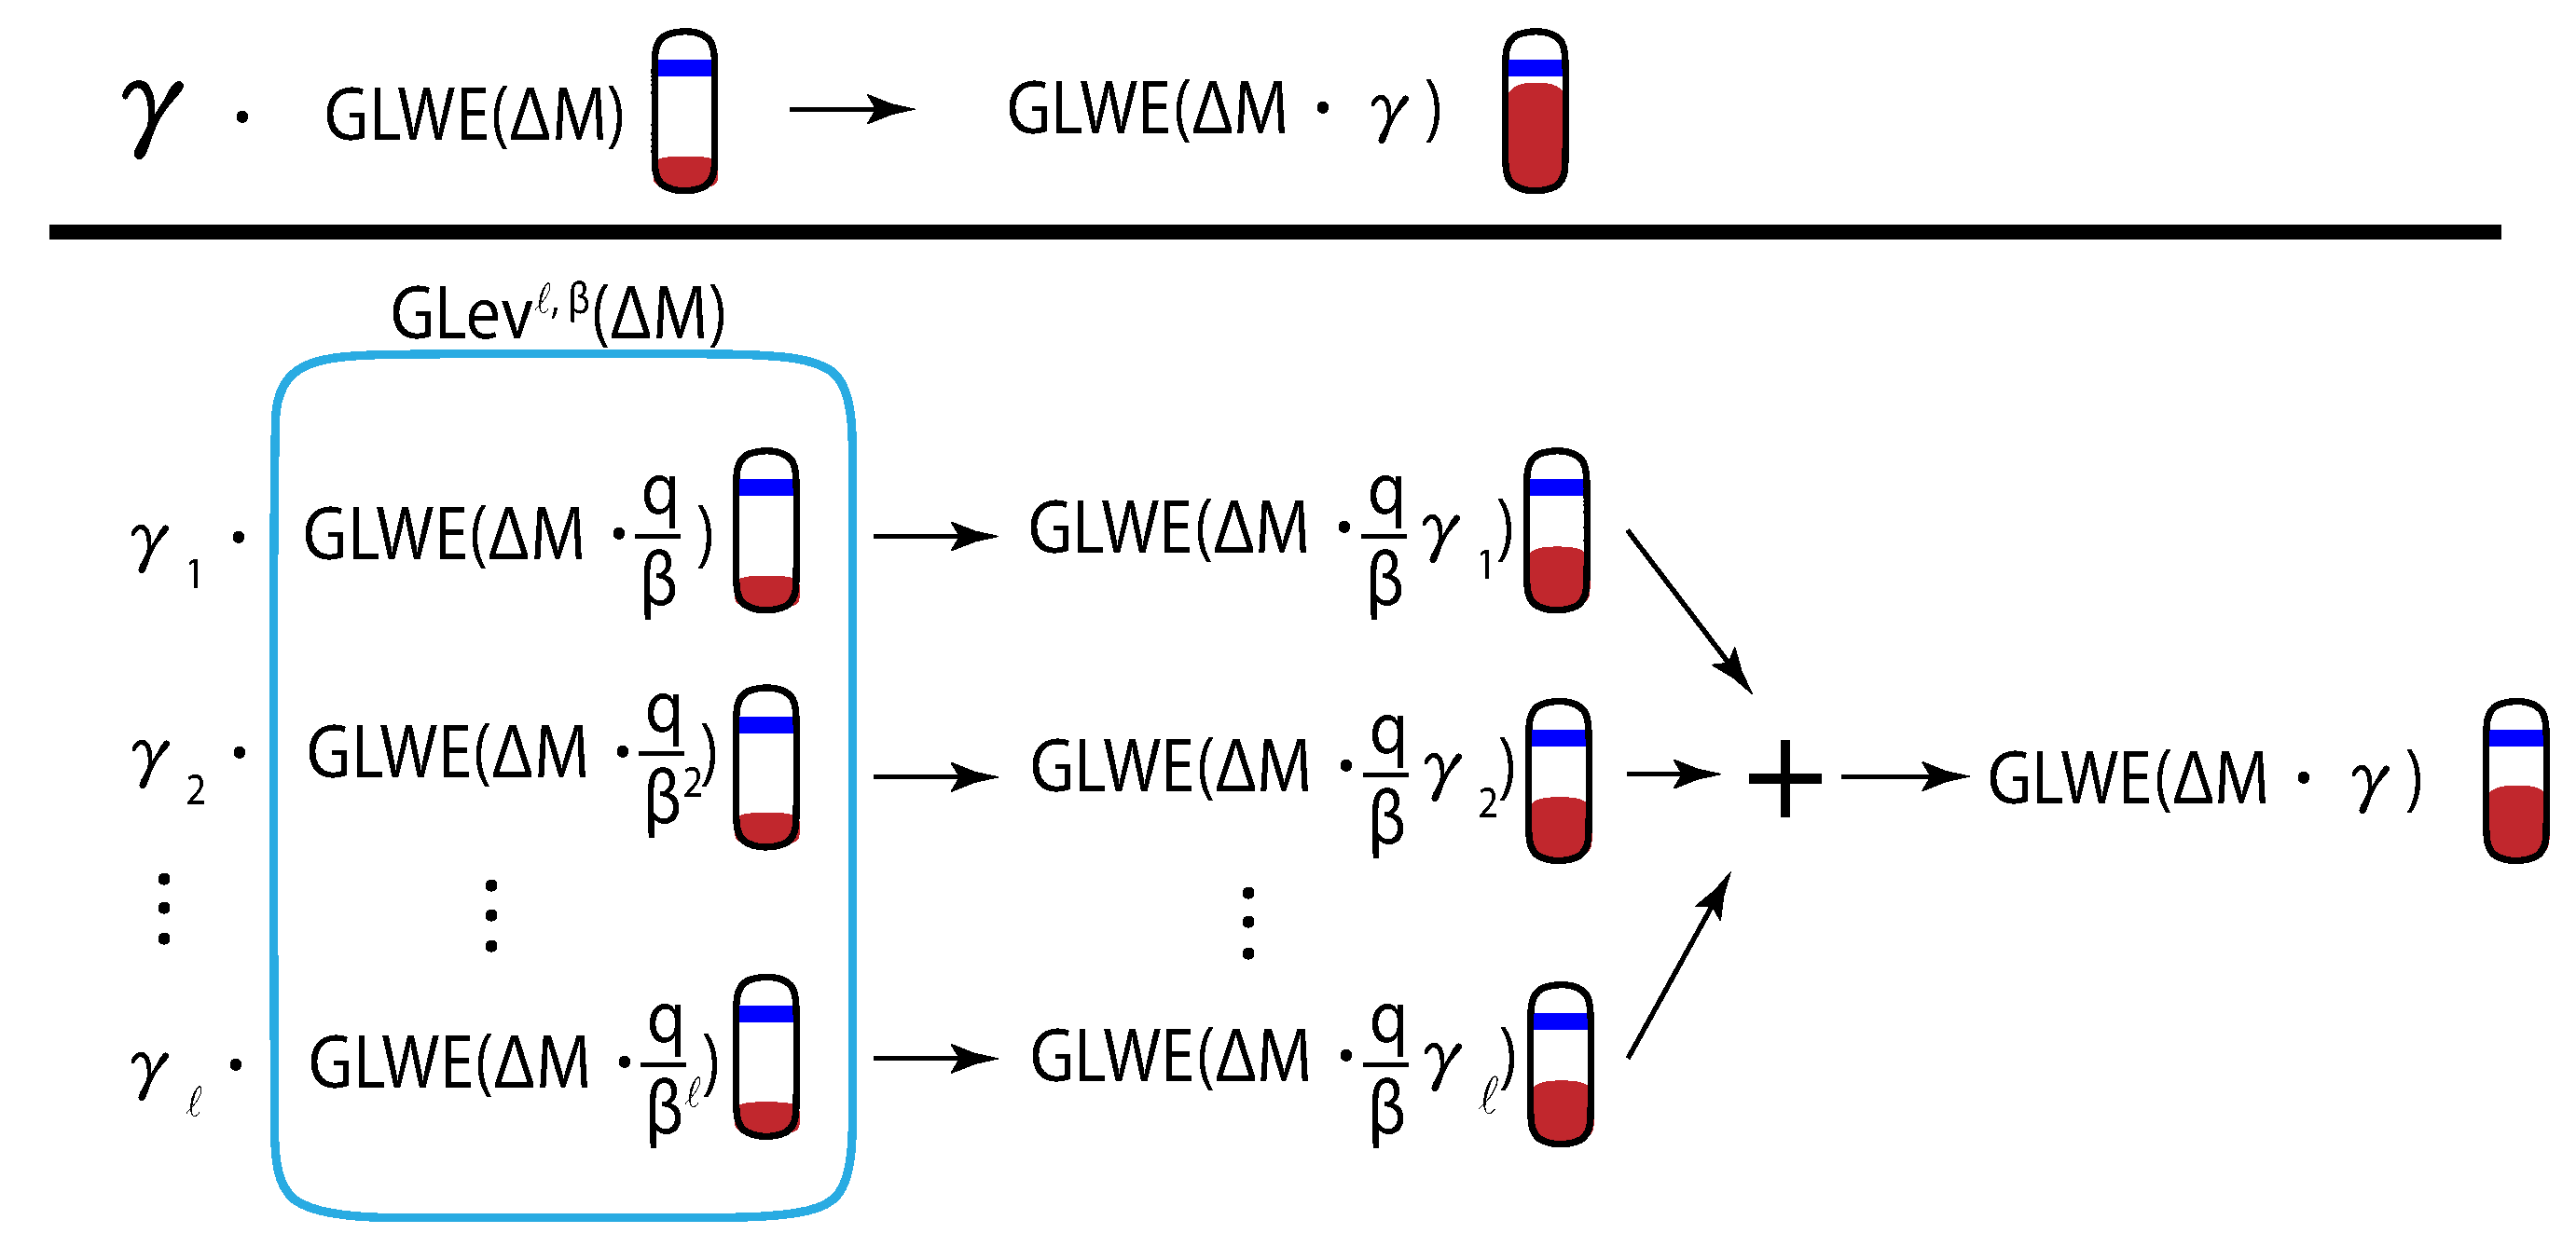
\includegraphics[width=0.8\linewidth]{figures/decomp2.pdf}
  \caption{Noise reduction in ciphertext-to-plaintext multiplication by gadget decomposition.}
  \label{fig:decomp2}
\end{figure}

However, we cannot use this decomposition technique to the resulting ciphertext again, because the output of this algorithm is a GLWE ciphertext and converting it into a GLev ciphertext without decrypting it costs much noise and computation time (as we need to multiply the GLWE ciphertext by $\dfrac{q}{\beta}, \dfrac{q}{\beta^2}, \cdots, \dfrac{q}{\beta^l})$.  

As a more efficient technique to re-initialize the noise $E$, we will describe TFHE's noise bootstrapping technique in \autoref{subsec:tfhe-noise-bootstrapping}.
